\clearpage
\section{Theoretical motivation\label{sec:theory}}


\subsection{The Standard Model\label{sec:SM}}

Particle physics concerns itself with the study of particles and the 
forces between them. Our current knowledge of their characteristics and 
interactions is formalized in the quantum field theory called the Standard Model 
(SM)~\cite{bettini2014introduction,griffiths2008introduction}.
It describes ``matter'' particles of spin-1/2 known as 
fermions. Six fermions of relatively small mass (leptons, $l$) are descibed:
The electrically charged electron ($e$), muon ($\mu$), and tau ($\tau$) 
leptons, and the electrically neutral and massless neutrinos 
$\nu_{e}$, $\nu_{\mu}$, $\nu_{\tau}$.  
Six other electrically charged 
fermions, named quarks, are in the Standard Model: up ($u$), down ($d$), 
charm ($c$), strange ($s$), top ($t$), and bottom ($b$). The quarks also carry
a charge analougous to the electric charge called color charge. Quarks in a 
free state have not been observed; they combine to make composite
particles called hadrons (e.g. protons, neutrons, pions). The masses of the 
fermions range from very small masses for neutrinos up to the heaviest 
particle described in the SM, the top quark, with a mass near 170 GeV. \\
\indent The interaction between these particles are mediated by spin-1 bosons: 
the massless and neutral photon $\gamma$ which mediates the electromagetic force, 
the massive $W^\pm$ and $Z^0$ that mediate the weak force, and the eight color 
charged, electrically neutral massless gluons which mediate the strong force.

\begin{figure}[h!t]
  \begin{center}
       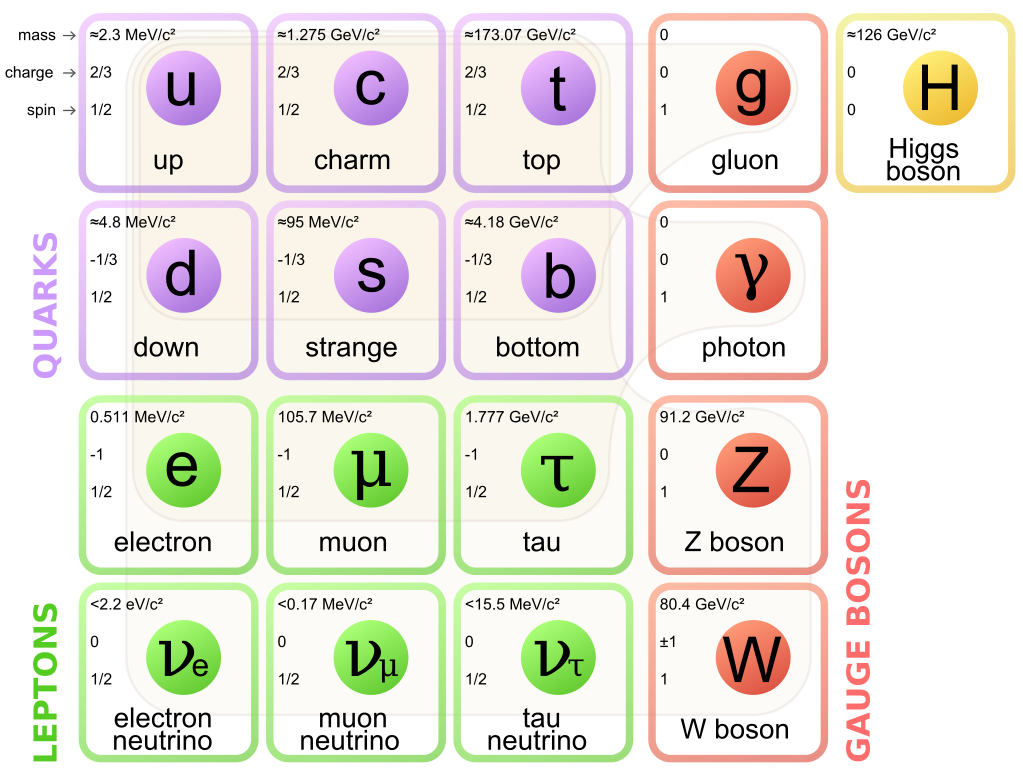
\includegraphics[width=0.85\textwidth,]{figures/Standard_Model_of_Elementary_Particles.png}
       \caption{The particles of the Standard Model.}
    \label{fig:SM-particles}
  \end{center}
\end{figure}

The interacations are governed by three symmetries of the SM: the color charge 
symmetry of Quantum Chromo Dynamics (QCD) represented in SU(3), the flavor 
symmetry of Quantum Flavor Dynamics (QFD) represented in SU(2) and the electric 
charge symmetry of Quantum Electro Dynamics represented in U(1). Together, SU(3) 
$\times$  SU(2) $\times$ U(1) requires the SM Lagrangian be invariant under 
local gauge transformations~\cite{perkins2000introduction}. The SU(2) $\times$ U(1) represent the electroweak interaction, 
which give rise to the photon, and the three weak gauge bosons: $W^{+}$, $W^{-}$ and $Z^0$.
%In the initial electroweak theory four massless bosons were introduced: $W^\pm$, $W^{0}$, $B^{0}$.
%Through the quantum numbers weak isospin $T$ and hypercharge $Y$, these bosons interact with all fermions.
The strength of the coupling between a boson and a fermion is determined by the 
charge belonging to the interaction. The quantum number weak isospin ($T$) is the charge 
of the weak interaction, and all interactions conserve the third component of weak isospin ($T_{3}$).
The electric charge ($Q$) can be represented by $T_{3}$ and the weak hypercharge ($Y$) 
corresponding to the U(1) symmetry:

\begin{equation}
\label{eq:Q-charge}
Q = T_{3} + \frac{Y}{2}
\end{equation}

Given the electroweak interaction is of the group SU(2) x U(1), there are four fields associated 
with it: $W_{1}$, $W_{2}$, $W_{3}$ of the SU(2) group where each index
corresponds to a component of the weak isospin space, and the isosinglet $B$ corresponding
to the weak hypercharge of the SU(1) group. These four objects, being vectors, require an index but it 
is dropped here for simplicity. The vectors $W_{1}$ and $W_{2}$ which result from the 
gauge invariance of the SU(2) group, mix to give rise to the $W^{\pm}$:

\begin{equation}
\label{eq:vector-boson}
W^{\left(\pm\right)}= \frac{1}{\sqrt{2}}\left(W_{1} \pm iW_{2}\right).
\end{equation}

The mixing of $W_{3}$ and $B$ give rise to the photon and $Z$ boson: 
$\gamma = B \cos \theta_W + W_{3} \sin \theta_W$  and $Z = W_{3}\cos \theta_W - B \sin \theta_W$ ,
where $\theta_W$ is the weak mixing angle. An exact symmetry does not allow mass 
terms in the Langrangian because they are not invariant under a gauge transformation. 
Since the gauge bosons of the weak interaction are not massless this symmetry is exact 
but broken. This symmetry breaking also gives mass to the fermions of the SM. To 
parametrize this symmetry breaking a doublet of scalar complex fields is introduced, the so-called
Higgs field:
\begin{equation}
\label{eq:higgs-field}
\phi = \binom{\phi^{+}}{\phi^{0}}
\end{equation}

the potential is:
\begin{equation}
\label{eq:higgs-potential}
V(\phi) = \mu^2|\phi|^2 + \lambda|\phi|^2
\end{equation}

If $\mu^2 < 0$ and $\lambda > 0$ this leads to a non zero vacuum expectation value. 
As the field is described by a complex doublet it possesses four degrees of freedom. 
Three yield the mass of the weak gauge bosons. Since the fourth degree of freedom is 
not absorbed by the massless photon it results in a neutral spin-0 boson whose couplings 
to the fermions are proportional to their masses. This boson is named the Higgs boson and
its existance was recently confirmed by the CMS and ATLAS experiments at CERN.
Figure~\ref{fig:SM-particles} show the particles described in the SM along with their properties.

\subsection{Shortcomings of the SM}
The agreement between experimental measurments and SM predictions make
the theory incredibly successful. For example, its prediction of the W, Z and Higgs boson
years (even decades) before their detection highlights its
predictive power. Another example, is the agreement between experimental measurment 
and prediction (to the \textit{billionth} decimal place) of the anomalous magnetic dipole 
moment of the electron. Yet, the SM is not a complete theory. The observation of neutrino oscillation in 
the late 90's forced the first ``Beyond the Standard Model'' (BSM) 
extension of the theory in order to give neutrinos mass~\cite{zuber2003neutrino}. 
Furthermore, gravitational interactions are not incorporated in the theory,
and therfore, at the scale which graviational forces become non-negligible 
($\approx 10^19~GeV$) the SM begins to falter. Additionaly, a theoretical 
framework explaining the dark matter in the universe is absent in the Standard Model.
But perhaps most importantly, within the SM, the Higgs mass is corrected by fermionic
loop interactions which depend quadratically on the scale of which new physics may enter.
The fact that this correction is quardatic in nature, and not logarithmic like for 
other particles, implies that for the newly measured Higgs mass of $\sim\!125~\gev$
either new physics enters at the scale of $\mathcal{O}$(1 TeV), or some new
mechanism is required to remove this quadratic divergence, $e.g.$ supersymmetry~\cite{Martin:1997ns}.

\subsection{Supersymmetry\label{sec:SUSY}}

Supersymmetry (SUSY) theory is an extension of the SM. For each fermion (or boson) in
the SM, a new supersymmetric boson (or fermion) is introduced. Theories that incorporate 
supersymmetry (SUSY) introduce a new symmetry between bosonic and fermionic states. 
A theory invariant under a transformation between these states is called supersymmetric.
A strong motivation for such a theory is that, by construction, the divergent terms
to the Higgs mass is removed; the corrective terms from fermionic loops are cancelled by 
opposite-sign supersymmetric loop terms and vice versa. 

\begin{figure}[h!t]
  \begin{center}
       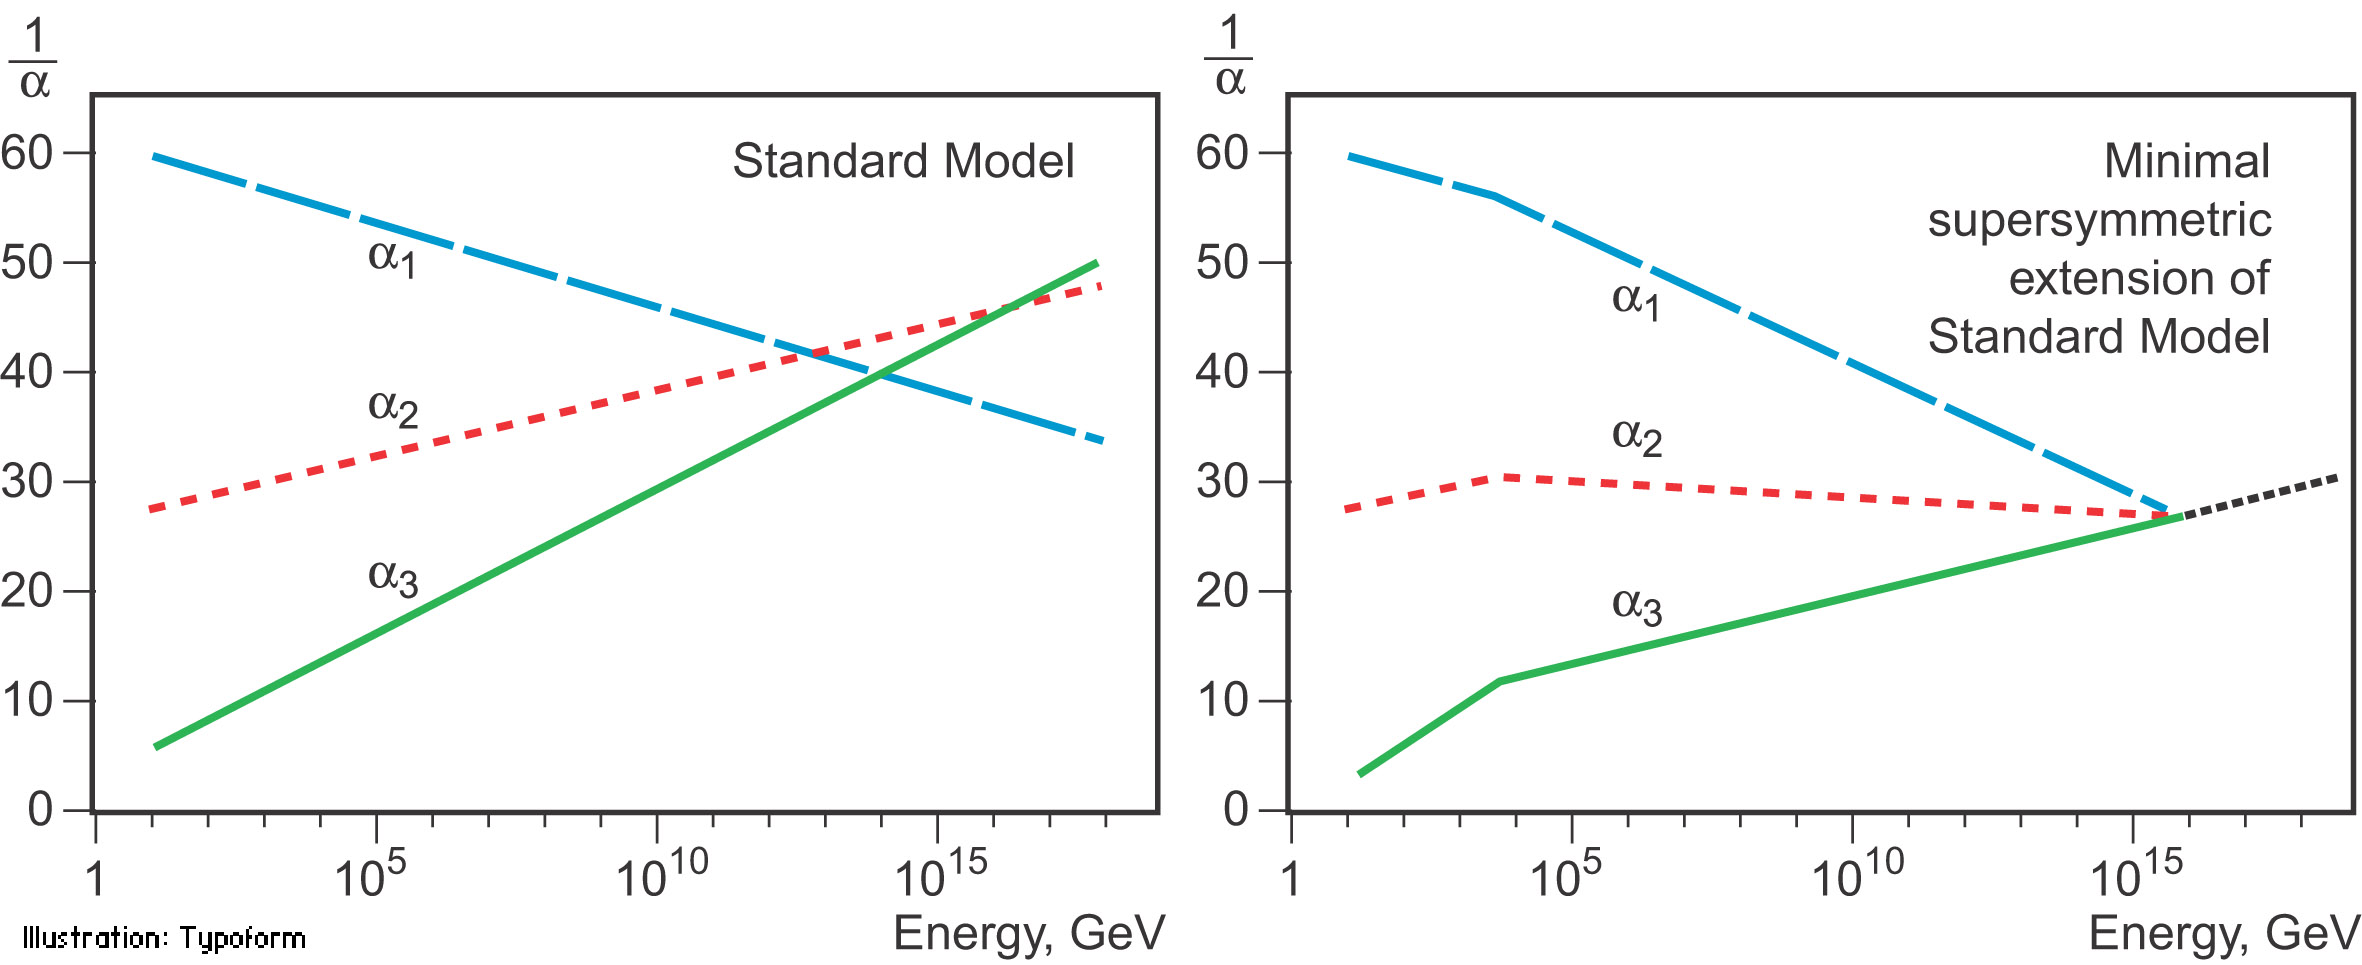
\includegraphics[width=0.65\textwidth,]{figures/phypub4highen.jpg}
       \caption{The particles of the Standard Model.}
    \label{fig:SM-particles}
  \end{center}
\end{figure}

The SM particle and its supersymmetric partner are identical in every quantum number except spin. 
The spin of the supersymmetric is derived from the spin of the SM particle $S_{m}$ by 
subtracting $\frac{1}{2}$ the exception being the Higgs boson which $\frac{1}{2}$ is added
to the spin.

%reasons. It allows for cancellation of quadratic divergences that appear in higher-order
%corrections to the calculation of the Higgs boson mass, because terms of opposite sign
%are contributed by the bosonic and fermionic superpartners. The
%lightest supersymmetric particle (LSP) in R-parity conserving models, described below, is usually neutral,
%massive, and weakly interacting, SUSY thus provides a candidate for dark matter. Finally,
%SUSY provides a mechanism whereby the coupling constants from the three standard model
%symmetry groups can be unified at a high scale, leading to the possibility of an even more
%fundamental theory, i.e., a “grand unified theory” (GUT)~\cite{wess1992supersymmetry}.\\
%\indent The theoretical underpinnings of SUSY rely upon a symmetry that relates bosons
%to fermions. In SUSY, the fundamental particle content of the universe will at least double,
%as all standard model particles will have a SUSY partner. 
%%For a minimal extension of the
%%standard model, the particle content, along with the relationship to standard matter, %is
%%shown in Table 2.1. 
%The scalar superpartners of the fermions are called sfermions and have a spin 0. The fermionic 
%superpartners of the bosons are called bosinos and half-integer spins. The names of the individual
%particles can be constructed in a similar manner.
%SUSY can be realized in many ways and it is important to choose a model that is
%consistent and yet feasible to study. A completely unconstrained minimal parametrization
%of SUSY contains over 100 free parameters. It is necessary to reduce the number of free
%parameters in order to effectively test the predictions of the theory, so certain assumptions
%are made to construct a consistent model with fewer free parameters. As superpartners
%have not yet been observed, their masses must be higher than the corresponding standard
%model particles. This necessarily means that SUSY is a broken symmetry, and the unknown
%mechanism providing the SUSY breaking can determine the type of physics one can expect
%to observe. Some commonly studied models, such as mSUGRA (minimal SUper GRAvity)
%and the cMSSM (constrained Minimal Supersymmetric Standard Model), posit that gravity
%is responsible for providing the SUSY breaking.
%
%\subsection{R-parity and a candidate for dark matter}
%
%R-parity, sometimes known as matter parity, is an additional symmetry (similar to
%the parity symmetry of the standard model) that determines the possible decays available
%in SUSY models. R-parity is defined in Equation~\ref{eq:r-par}, where B is the baryon number, L is the
%lepton number, and s is the spin of the particle in question. R-parity is a multiplicative
%quantum number, with R = 1 for ordinary standard model particles and R = -1 for SUSY sparticles.
%
%\begin{equation}
%\label{eq:r-par}
%R = \left(-1\right)^{3B+L+2s}
%\end{equation}
%
%R-parity-conserving models are preferred due to consequences of R-parity violating (RPV)
%models, which allow for the decay of the proton, among other currently unobserved decays. 
%While RPV models are not excluded, current theoretical prejudice favors R-parity 
%conserving models.
%If R-parity is conserved, this necessarily implies that a sparticle must be produced
%in conjunction with another sparticle, i.e., sparticles will always pair produced at collider
%experiments. Another consequence is that the LSP must be stable. Additionally, if the LSP
%is neutral, it will be noninteracting and thus a good candidate for cold dark matter. The
%neutral LSP is preferred in many models being explored at the LHC due to cosmological
%constraints on exotic matter~\cite{wess1992supersymmetry}.
%
%\subsection{Experimental signature}
%\label{sec:signature}
%
%Color confinement in QCD prohibits the isolation of quarks~\cite{Ellis:1991qj} 
%and as such, when a high energy quark is produced, e.g. 
%from a collision of other particles, it quickly fragments into a 
%color-neutral hadron. If the quarks in the hadron have enough energy, 
%they fragment again into other hadrons. This hadronization process 
%continues until the resulting particles are of low enough energy that it
%is no longer energetically favorable to fragment. The hadronic shower of
% particles can be clustered into objects called ``jets''. A simulation 
%of such a jet is shown in Figure~\ref{fig:jets}.  
%
%\begin{figure}[h!t]
%  \begin{center}
%       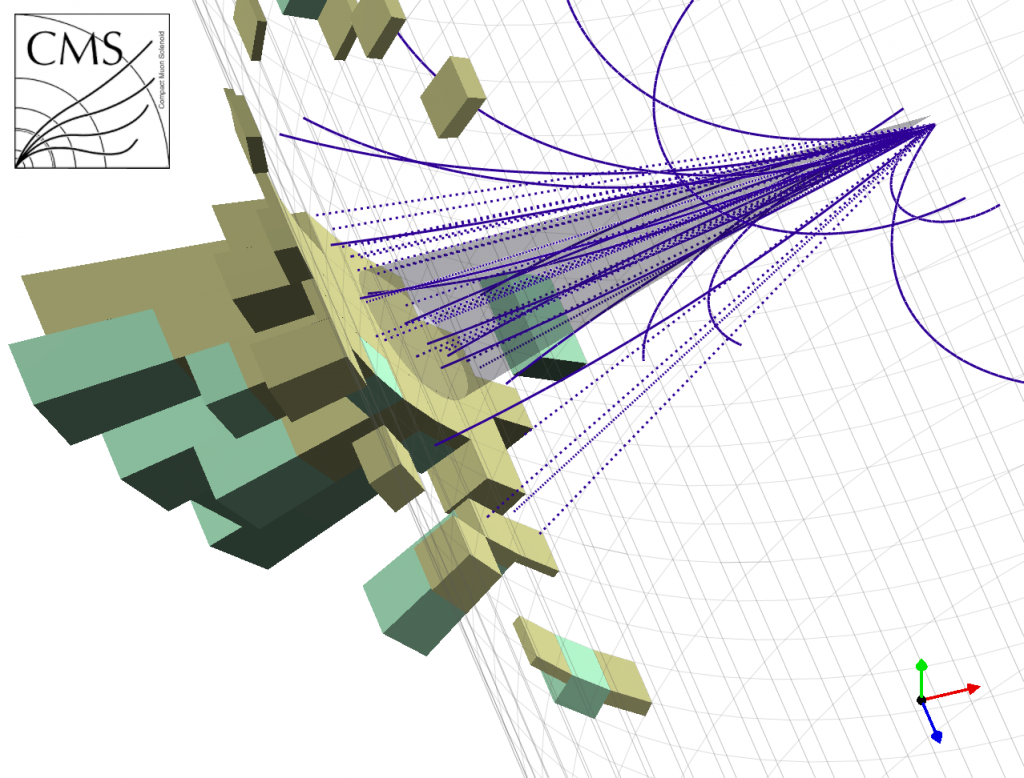
\includegraphics[width=0.45\textwidth,]{figures/JetConeAndPFJet.png}
%       \caption{A simulation of a hadronized quark in the CMS detector. The
%       resulting particles from hadronization are grouped into a jet (gray cone). }
%    \label{fig:jets}
%  \end{center}
%\end{figure}
%
%In this analysis, a search for excess in events consisting of jets and 
%missing energy is conducted. This final state is expected when pairs of
%heavy squarks or gluinos are produced and decay hadronically to SM quarks,
%gluons, and neutralino, which escape the detector leaving only a signature
%of missing energy.
%%Such an excess would not directly validate a 
%%supersymmetric extension of the Standard Model, since other interpretation are 
%%possible, but nonetheless supersymmetry provides a extensive framework for interpretation. 
%The full unconstrained SUSY theory is parametrized by over 100 variables, representing 
%masses, phases and mixing angles, but it can be simplified. These simplified supersymmetric 
%models (SMS) are limits of more general new-physics scenarios, where all but a few 
%particles are integrated out~\cite{Alves:2011wf}.
%The dominant contribution to the divergence of the Higgs boson mass arises from 
%loop diagrams involving the top quark; these can be largely canceled if a scalar 
%partner of the top quark (top squark) exists and has a mass below 
%$\sim\!\!1\TeV$~\cite{Alves:2011wf}.
%This relatively low mass is a motivation to interpret the results of this 
%analysis in two decay channels of the direct pair-produced top squark. 
%In the first channel, where the top squark decays to a top quark (followed by a 
%semi-leptonic decay: $t \ra Wb \ra l \nu b$), provides the highest reach in probing the mass
%of the top squark. The second decay scenario has only been recently pursued. It puts 
%the mass difference between the top squark and the neutralino at 80~\GeV or 
%less, resulting in the top squark decaying directly into a charm quark. 
%Figure~\ref{fig:feynman_sms} shows the schematic diagrams of these two decay channels. 
%More detailed description of each model is left for Section~\ref{sec:signal}
%
%\begin{figure}[ht!]
%  \begin{center}
%    \subfigure[\label{fig:feyn_t2tt}]{
%      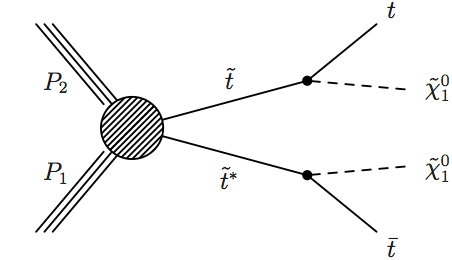
\includegraphics[width=0.45\textwidth,]{figures/T2tt}
%    } 
%    \subfigure[\label{fig:feyn_t2cc}]{
%      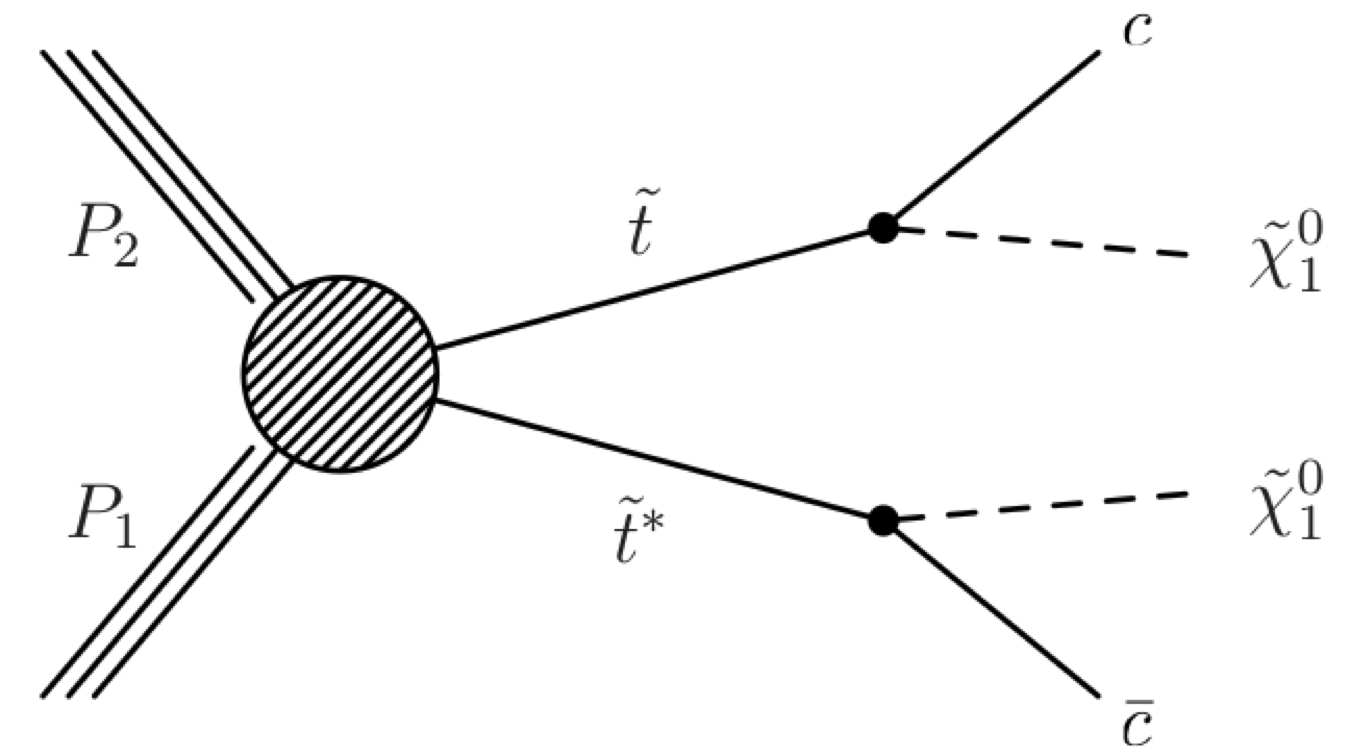
\includegraphics[width=0.45\textwidth,]{figures/T2cc}
%    } \\
%      \caption{Two Feynman diagrams depicting the top squark production
%      and decay, in which P represents a proton, $t$ a top quark, $c$ a charm
%      quark, $\st$ a top squark, \chiOnez a neutralino.}
%    \label{fig:feynman_sms}
%  \end{center}
%\end{figure}
%
%%\begin{figure}[ht!]
%%  \begin{center}
%%      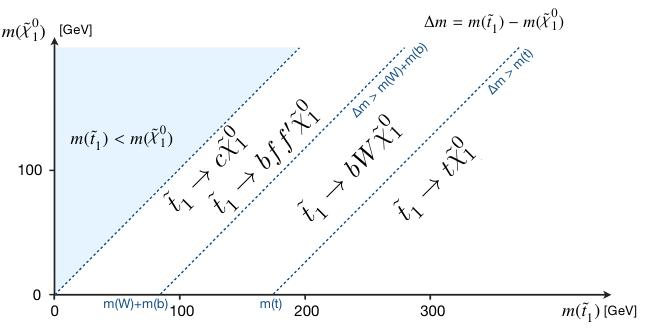
\includegraphics[width=0.45\textwidth,]{figures/mstop_mLSP_plane.jpg}
%%      \caption{}
%%    \label{fig:mStop_mLsp.jpg}
%%  \end{center}
%%\end{figure}
